\chapter{Results and Discussion}\label{cp:res}
This chapter highlights the important results of the project. It starts off discussing the outcomes of preliminary tests that were done offline with prerecorded data using python. Next, the implemented software is evaluated against the results from python, Korotkoff sounds and by doing repeated measurements. 


\begin{figure}[ht]
\centering
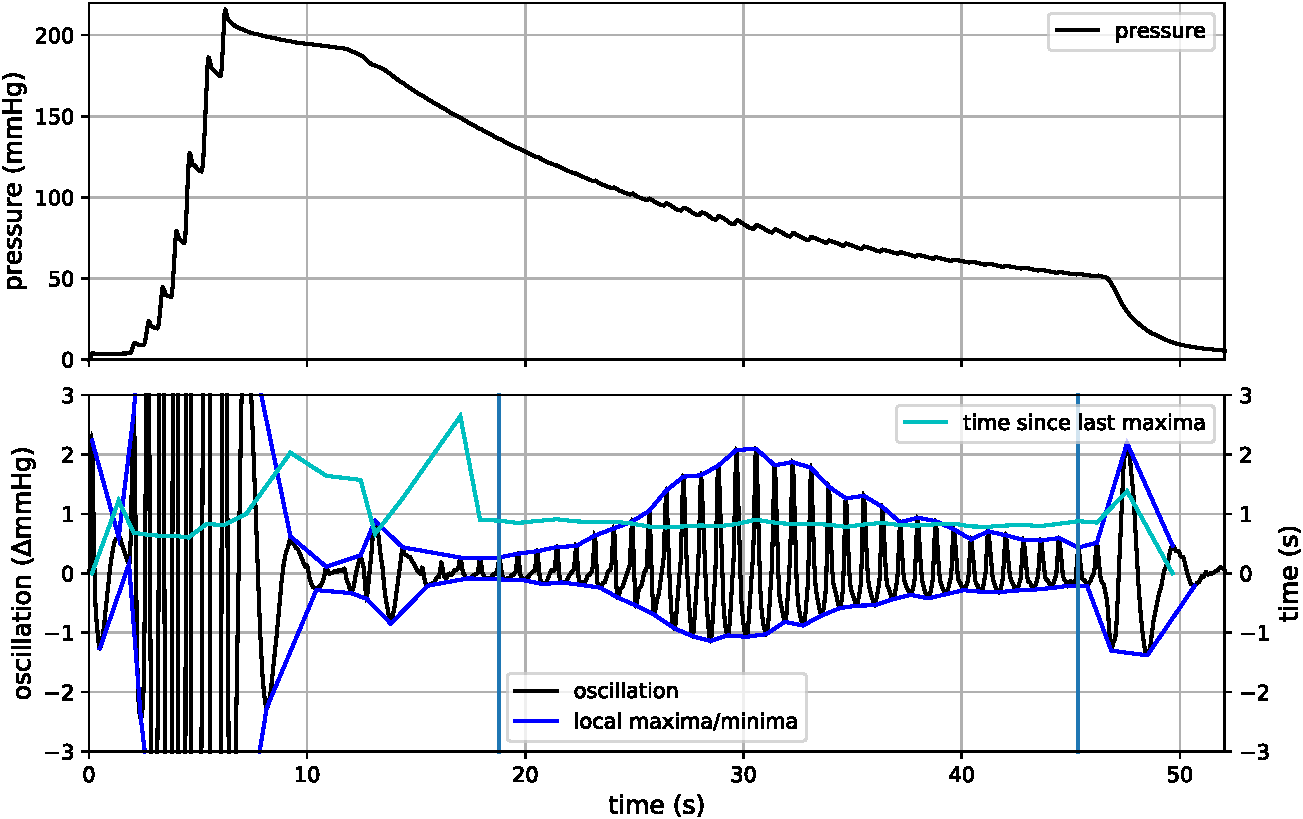
\includegraphics[width=\textwidth]{figures/mmHg_Signal.pdf}
\caption{Processing of a dataset. The top plot shows a dataset, and the bottom one shows how it is analysed by identifying the extrema and comparing the time between maxima..}
\label{fig:pyOverview}
\end{figure}

\section{Python Algorithm Tests}
Before deciding on an algorithm to implement, some test data was recorded and analysed offline using python. Different approaches of the MAA were implemented as well as the derivative algorithm. All python tests are done on the same dataset. The manually determined blood pressure was 110/70, with a large, expected error because the pressure was taken by an untrained person on themselves. 

The top plot in figure \ref{fig:pyOverview} shows the by now familiar outline of a BP measurement. The bottom plot illustrates how it was analysed. The oscillations were examined for local extrema and the resulting points connected for the maxima and minima. The result is the blue line that forms the envelope around the oscillations. The cyan line is the time difference between two subsequent maxima. From this, the heart rate can be calculated. It is used to determine when to analyse the oscillations. When the heart rate is stable and changes less than \SI{20}{\percent} per detection, the start of the oscillometric envelope is assumed. When it changes dr, the end is recognised. These points are identified in the bottom plot in figure \ref{fig:pyOverview} by the vertical lines. 

\subsection{Fixed-Ratio Algorithm}\label{sec:pyfixed}

Figure \ref{fig:pyFR} shows the same data as before but analyses only the part between the vertical axes in figure \ref{fig:pyOverview}. The plot shows the different ways the OMWE can be calculated. They have been normalised for comparison. The blue trace is simply the detected maxima connected. Every minimum subtracted from its preceding maximum is the green track. For the red trace, interpolation is done between each of the detected maxima and the equivalent for the minima. The subtraction of the resulting minima from the maxima is the red trace. Finally, the purple curve is a polynomial of \nth{4} order fit to the points calculated in the green track. 

\begin{figure}[ht!]
\centering
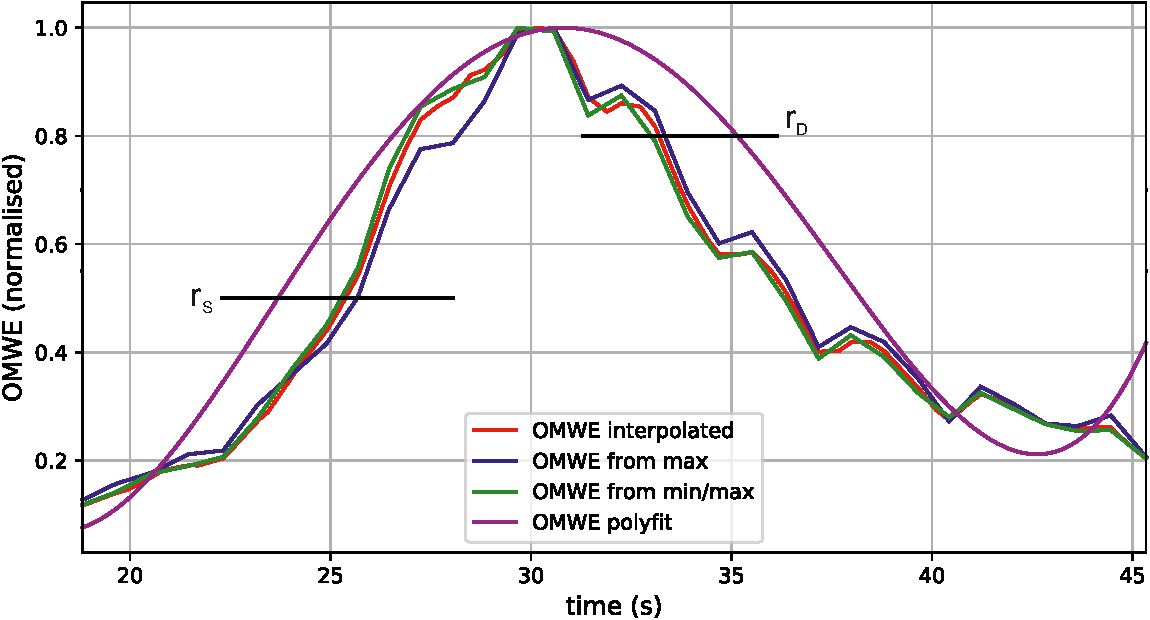
\includegraphics[width=0.9\textwidth]{figures/OMWE_normalised.pdf}
\caption{Ways to form the OMWE. The plot shows different ways to calculate the OMWE, normalised by their maximal value for comparison. Vertical lines are drawn at $r_S =0.5$ and $r_D=0.8$, where SBP and DBP are assumed.}
\label{fig:pyFR}
\end{figure} 

MAP is determined  where the envelopes have their maximum as explained in chapter \myref{sec:MAA}. Vertical lines are drawn at $r_S=0.5$ and $r_D=0.8$ where SBP and DBP are estimated in this example.


Table \ref{tbl:maacomp} lists the values for MAP, SBP and DBP that were calculated for each of the OMWE formation methods. 

\begin{table}[ht!]\label{tbl:maacomp}
\centering
\begin{tabular}{lllll}
\hline
           & max value & min/max value & interpolation & polynomial fit \\ \hline
MAP (mmHg) & 82.64     & 85.50         & 82.49         & 81.53          \\ 
SBP (mmHg) & 97.21     & 98.83         & 99.14         & 105.63         \\ 
DBP (mmHg) & 73.04     & 72.64         & 71.83         & 66.53          \\ \hline
\end{tabular}
\caption[Comparison of different methods to form the OMWE on the calculated BP values for the MAA.]{Comparison of different methods to form the OMWE on the calculated BP values for MAA. MAP was estimated at the maximum of the OMWE, SBP at a ratio of 0.5 of the maximum while rising and DBP at a ratio of 0.8 of the maximum while falling.}
\end{table}

All methods estimate MAP within a range of \SI{4}{\mmHg}. The furthest off is the min-max OMWE (green). Small shifts in time influence it because minima are happening after maxima. Surprisingly, the OMWE using only the maximum values (blue) estimates MAP closer to the other methods. However, while oscillations are increasing and decreasing, the blue trace shown in figure \ref{fig:pyFR} seems to lag behind the others in time, and SBP is therefore estimated slightly lower, with \SI{97}{\mmHg}. DBP is not determined lower, with \SI{73}{\mmHg}, although it is happening later. This is due to a pulse peak occurring in the deflating data and a weakness in the python script. It estimates the values at their exact position in the deflating plot without taking into consideration the small pulses that are still occurring there (see figure \ref{fig:pyOverview}, top plot).

The purple polyfit trace does a decent job identifying MAP, but the trail hardly fits the envelope. As is shown in figure \ref{fig:pyFR}, it is wider than the other methods. Therefore, it estimates SBP sooner and DBP later, resulting in a considerably higher value for SBP with \SI{106}{\mmHg} and a lower value for DBP with \SI{66}{\mmHg}. 

The green OMWE that is considering minima and maxima is similar to the red interpolation one from \SIrange{23}{27}{\s}. Looking back at figure \ref{fig:pyFR}, maxima are followed quickly by minima in this period. The way this trace is calculated explains why it is slightly shifted backwards in time compared to the red one: The values are evaluated when the maxima happen, and the following minimum is subtracted from it. During deflation, the time difference between extrema increases and the curves differ increasingly.

Altogether, the red interpolation trace looks the most continuous. Changes in timings of minima and maxima have the least effect on it. 

Finally, the determination of the pressure at the identified time should be done by averaging over the current pulse and not by evaluating the given sample directly from the low-pass filtered deflation curve.

\subsection{Derivative Algorithm}\label{sec:pyder}
The same data was used to test the derivative algorithm. The oscillation data plotted in time is shown again in figure \ref{fig:pyDer} on the left-hand side. The top is the deflating pressure and the bottom the shows the oscillations.

The right-hand side shows the oscillations plotted in terms of pressure when they were happening. Note that this changes the x-axis and the resulting plot is an inversion in time. The lower pressures occurred later than the higher pressures. 

\begin{figure}[ht!]
\centering
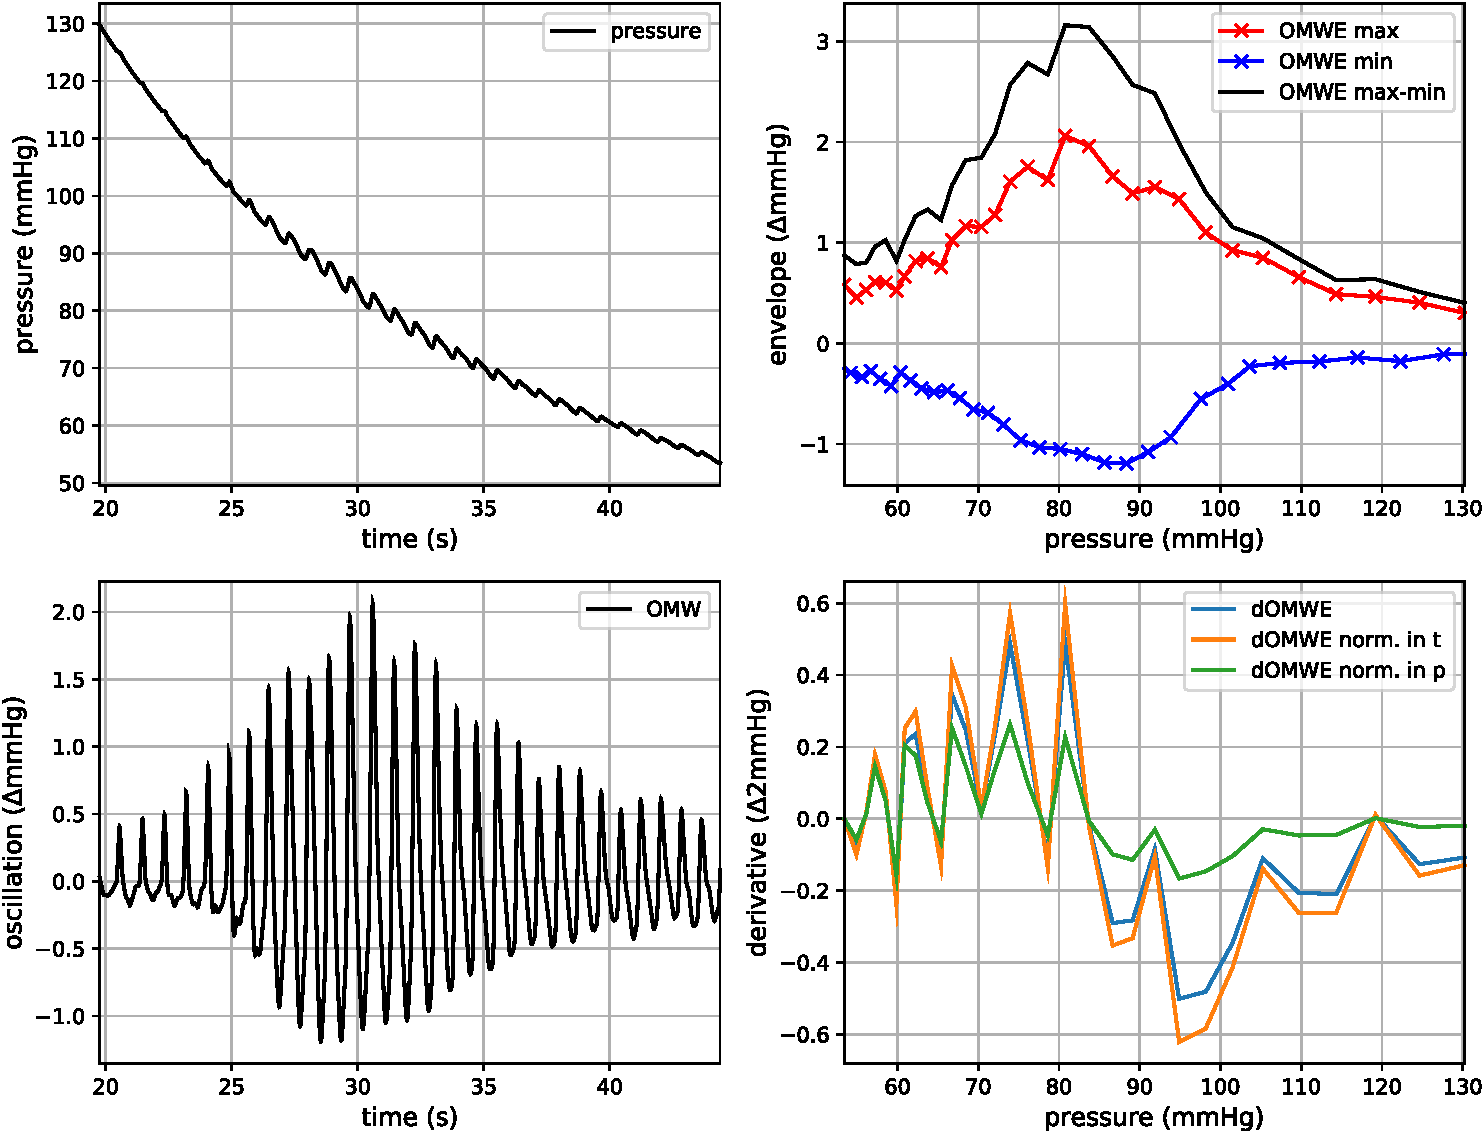
\includegraphics[width=\textwidth]{figures/derrivative_envelope.pdf}
\caption{The derivative algorithm is tested with python. The left-hand side shows the known plots of deflating pressure (top) and oscillations (bottom). The right-hand side shows the formation of the OMWE on the top. Note that the x-axis is the pressure when the oscillations occurred. The bottom right is the derivative of the OMWE normalised in different ways.}
\label{fig:pyDer}
\end{figure} 

The plot on the top right shows how this OMWE is formed from the detected maxima and minima. The bottom-right plot shows the derivative of the OMWE. The blue trace is the difference between two successive data points. Because they are spaced unevenly, the orange trace has the values normalised by the time difference between them. The green track normalises the derivatives with the pressure difference. While the green curve seems to make the most sense logically, they all look similar, except for the green one being compressed compared to the others. A variation of this figure, where all derivative traces have been normalised by their maximal value for comparison, can be found in the appendix.
%TODO put figure in appendix and reference here 

Taking the maximum value of the derived OMWE results in the DBP and the minimum value in the SBP, as explained in section \myref{sec:der}.
Table \ref{tbl:pyDer} lists the values for SBP and DBP that were computed for each of the OMWE methods. SBP is identified at \SI{94.87}{\mmHg} and DBP at \SI{80.87}{\mmHg} or \SI{73.94}{\mmHg}. The only difference in the three approaches is the DBP that is estimated lower by the derivative that was normalised in pressure. The lower is most likely the closest to the actual value because it relates to the one determined with the fixed-ratio algorithm.

\begin{table}[t]\label{tbl:pyDer}
\centering
\begin{tabular}{llll}
\hline
           & not normalised & normalised in time & normalised in pressure \\ \hline
SBP (mmHg) & 94.87          & 94.87              & 94.87                  \\ \hline
DBP (mmHg) & 80.76          & 80.76              & 73.94                  \\ \hline
\end{tabular}
\caption{Comparison of blood pressure values calculated by the derivative algorithm for differently normalised derivatives.}
\end{table}


Other tests, using only the maxima or minima for derivation, have produced plots that are even more ambiguous. For this particular example, the minima are smooth, and the derivative had a clear indication for the SBP. The plots for this test are located in the appendix.
%TODO minima in appendix

Additionally, it has to be noted that the tests were done using an immaculate data set. If the deflation curve is not as stable as in the example, the derivative algorithm does not work at all. Similarly, even if the deflation is steady, but there are any other artefacts in the oscillations, e.g. from micromovements or natural blood pressure variations over time, the wrong blood pressure will be measured. Figure \ref{fig:pyDer2} in the appendix shows the same algorithm using non-ideal data that was recorded within minutes of the data shown above. All methods determined  SBP at \SI{84.65}{\mmHg} and systolic DBP at \SI{62.58}{mmHg}. Both values are \SI{10}{mmHg} lower compared to the previous measurement analysed by both the derivative and the fixed-ratio algorithm. 
%TODO appendix
%\begin{figure}[ht!]
%\centering
%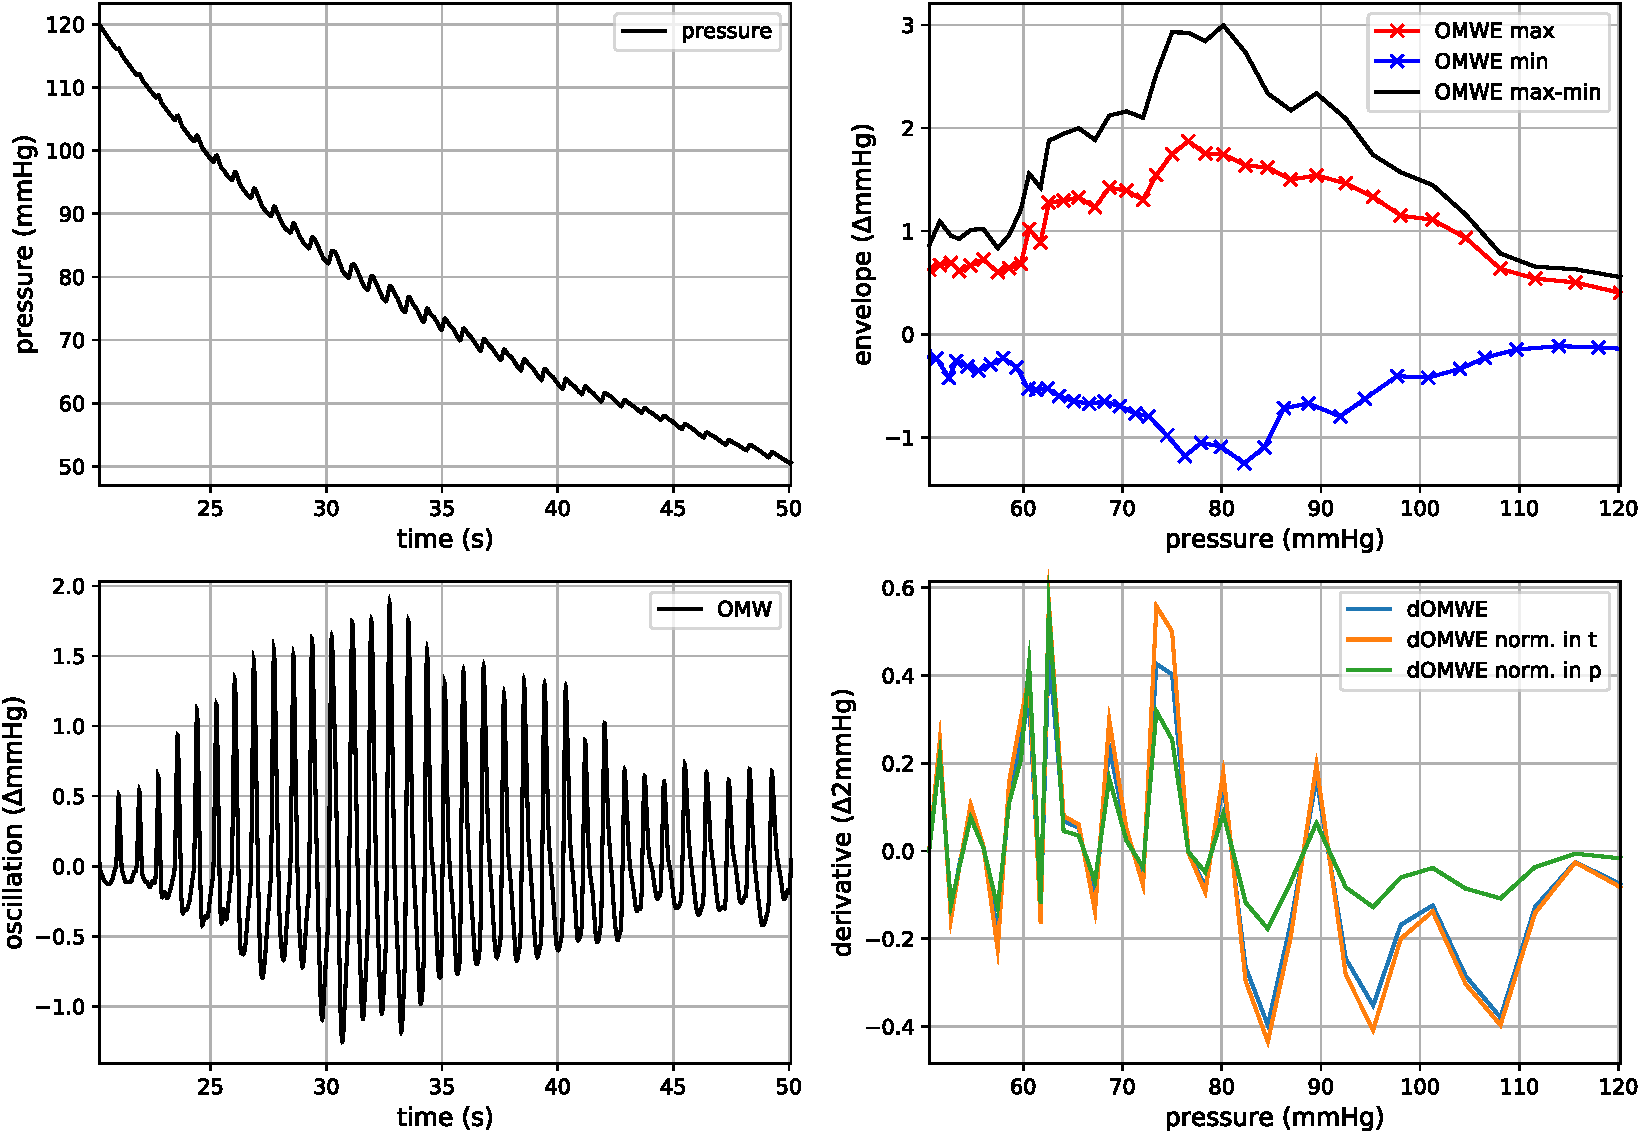
\includegraphics[width=\textwidth]{figures/derrivative_measurement2.pdf}
%\caption{A second measurement, taken within minutes of the first, results in a very different derivative graph.}
%\label{fig:pyDer2}
%\end{figure} 


\subsection{Summary}

\begin{table}[ht]\label{tbl:sumPy}
\centering
\begin{tabular}{lll}
\hline
           & fixed-ratio interpolated & derrivative normalised in pressure\\ \hline
MAP (mmHg) & 82.49       & -           \\ \hline
SBP (mmHg) & 99.14       & 94.87       \\ \hline
DBP (mmHg) & 71.83       & 73.94       \\ \hline
\end{tabular}
\caption{Comparison of blood pressure values calculated by the fixed-ratio and the derivative algorithm.}
\end{table}


Table \ref{tbl:sumPy} lists the values of the results from the two best options for the fixed-ratio and derivative algorithm. For the fixed-ratio algorithm, the interpolated version is chosen because it has the smoothest curve. The derivative algorithm is logically and in the current measurement best for the version normalised in pressure. However, even using clean data that is optimal for the derivative algorithm, the values have little confidence.  There is no apparent rising and falling curve that has a distinct maximum and minimum, but rather an assembly of maxima and minima. Even the smallest changes in amplitude or time difference have a significant impact on the results. Therefore, this approach is not implemented in the application.

As expected, the fixed-ratio algorithm produced stable estimates of MAP. Of course, it also depends on how the OMWE is defined. The interpolated version has the least sensitivity to noise because it considers the time difference between minima and maxima. SBP and DBP are highly dependant on the chosen ratios. For this test, the ratios were selected as recommended by \citet{Geddes1982} ($r_S =0.5$ and $r_D=0.8$).



\section{Application Implementation}
To assess the results,  C++ calculations are compared to python. Next, Korotkoff sounds are compared to the OMWE. Finally, a series of measurements are made within a short period to test reproducibility.


\subsection{Comparison to Python Algorithm}
To make sure the in C++ implemented algorithm does what it is expected to, a measurement is performed and compared against the python algorithm. From the application, not just the raw data was saved, also low and high-pass filtered data and the OMWE that is used by the algorithm were written to a file. The raw data was analysed by the same python script described above (section \myref{sec:pyfixed}). The filtered and calculated data from the application is plotted over it in figure \ref{fig:comp}. The used filters are the same and perform correctly, as can be seen in the pressure plot at the top and the oscillation plot in the middle. 

\begin{figure}[ht!]
\centering
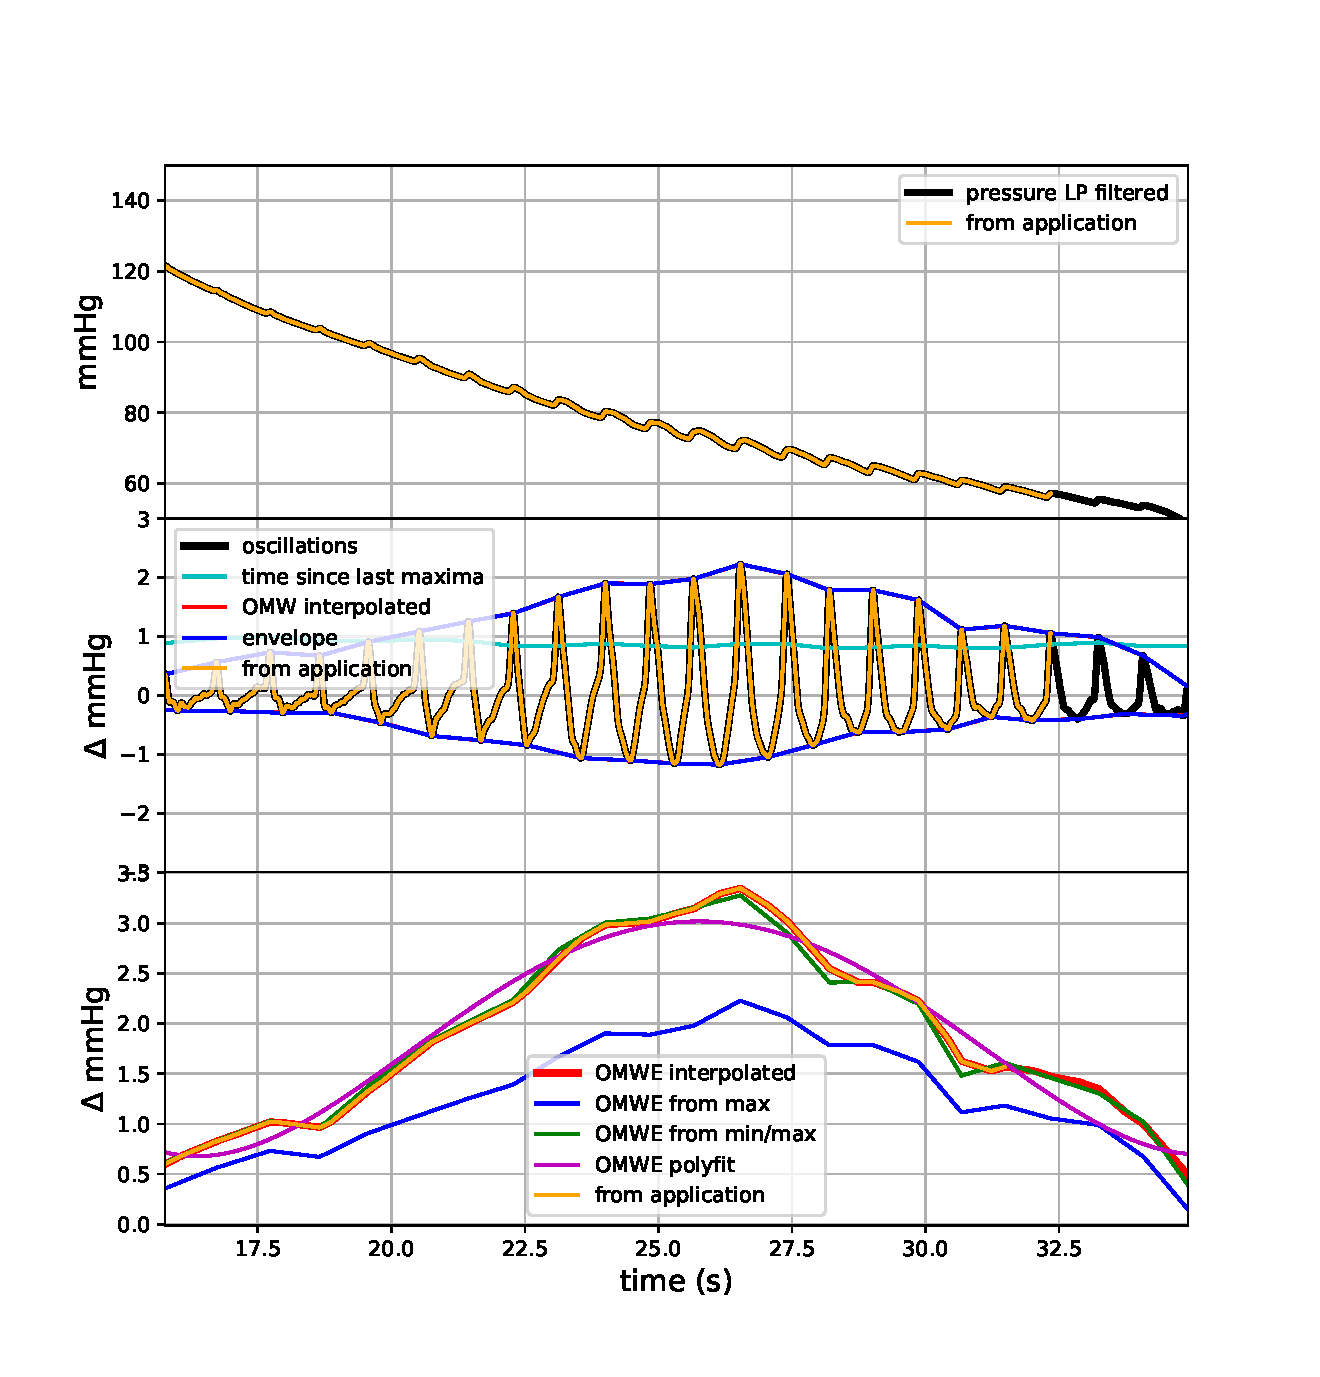
\includegraphics[width=\textwidth]{figures/compare_proces_signal.pdf}
\caption{...}
\label{fig:comp}
\end{figure} 

The bottom plot shows the OMWE calculated by the application matches the interpolated version in python. Because interpolation is done linearly in python, only calculating the edge values results in the same trace as the fully interpolated version, with considerably fewer computations.


\begin{table}[b]\label{tbl:sumAlgo}
\centering
\begin{tabular}{lll}
\hline
           & C++ Application & Python Script\\ \hline
MAP (mmHg) & 71	             & 71.87        \\ \hline
SBP (mmHg) & 95              & 94.50        \\ \hline
DBP (mmHg) & 67              & 66.05        \\ \hline
\end{tabular}
\caption{Blood pressure values calculated by the C++ application and the python script from the same data.}
\end{table}

Table \ref{tbl:sumAlgo} shows the calculated values for the python and application implementation. The difference is that the application uses an average pressure value around the determined time, whereas the python script directly looks up the pressure value at the given time. 



\subsection{Korotkoff Sounds}\label{sec:koro}

Figure \ref{fig:audio} shows a test where a stethoscope was placed under the cuff to record Korotkoff sounds while performing the measurement. The resulting values are; \SI{109}{\mmHg} for SBP, \SI{77}{\mmHg} for MAP and \SI{71}{\mmHg} for DBP with an average heart rate of \SI{74}{beats/\minute}. Korotkoff sounds only allow estimations of DBP and SBP.


\begin{figure}[ht!]
\centering
\includegraphics[width=\textwidth]{figures/audio2.pdf}
\caption{...}
\label{fig:audio}
\end{figure} 

In figure \ref{fig:audio}, the green arrows are linked to the OMWE, which is displayed normalised to identify the ratios. As before, the values are 0.5 for $r_S$ and 0.8 for $r_D$. \circled{1} shows where the algorithm expects systolic pressure and \circled{2} diastolic pressure. The orange arrows relate to the sounds displayed in the central plot. \circled{3} is where the sounds first appear, \circled{4} where they are muffled and \circled{5} where the sounds disappear entirely. According to \cite{Boron2012}, DBP is located where the sounds are muffled. This point is difficult to see in the plot, but easy to hear. It corresponds well with the ratio of 0.8 for this measurement.
Because the ratios are known to be dependant on factors like age and health, the software allows to change them in the settings.  On the other hand, if the guidelines are followed that DSP is located where Korotkoff sounds disappear \citep{Lloyd2018,Reeves1995}, the ratio should be less than 0.5. 



Altogether, the chosen ratios work decently. According to \citet{Sapinski1996}, the auscultatory method underestimates SBP and overestimates DBP, which fits with our findings. However, the ratios are known to be highly dependent on BP, age and health of the subject and the pressures calculated from them should only be used as indications and not fixed values. 

\subsection{Repeated Measurements}
Unfortunately, the ethical application to perform experiments with test subjects was rejected given the current circumstances. Therefore, the only tests were performed on the developer. 

\begin{figure}[ht!]
\centering
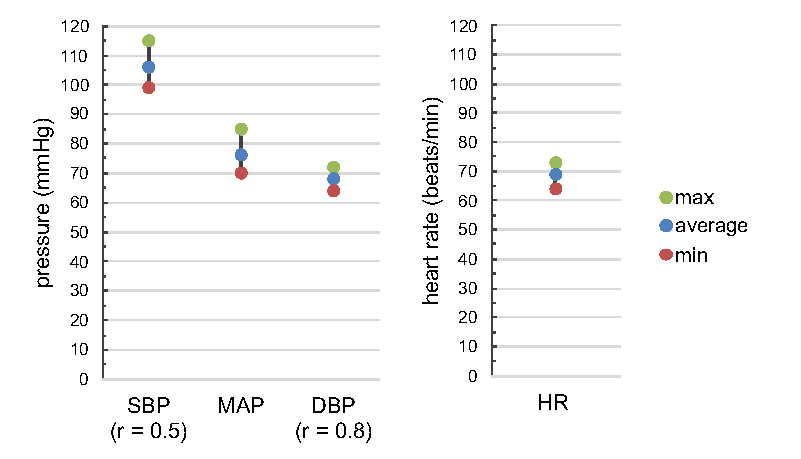
\includegraphics[width=0.85\textwidth]{figures/measurements.pdf}
\caption{...}
\label{fig:rep}
\end{figure} 

Figure \ref{fig:rep} shows how the measured values vary in a period of twenty minutes, performing ten measurements in a row. The ratios for systolic and diastolic BP were 0.5 and 0.8. For each determined value type, the maximal, minimal and average is indicated. The individual measurements can be found in the appendix. Besides MAP, DBP and SBP, the heart rate was noted as an indicator of natural variations. The heart rate is the signal that can be registered most accurately. Both MAP and SBP have significant differences of \SI{16}{\mmHg} and \SI{15}{mmHg}. The heart rate and DBP vary less than \SI{10}{\mmHg}. For the DBP, this is surprising. The research with python has shown that irregularities in amplitude are more common in the diastolic range. One explanation is because oscillations decline quicker than they increase, the pressure range is smaller for DBP. However, this explanation is based on subjective observations and might be misleading. 

A manual blood pressure measurement was performed before and after the automatic ones. Before, BP was determined at 110/80 and after at 100/70. These should only be used as a reference and not as the 'right' values. The tester performed them on themselves, with the stethoscope tucked under the cuff, which is known to influence the measurement. Additionally, the person is not trained to take BP. 

Still, it shows that it is likely that the average blood pressure dropped within the twenty minute time frame, which can account for part of the variations.

All tests were successful because the tester/developer knows what to pay attention to during a measurement. Experiments with untrained people would have been interesting. It would also have provided feedback on the usability of the GUI, and if it guides the user sufficiently, so they can take successful measurements. 